%\documentclass[twocolumn,10pt]{IEEEtran}
\documentclass[conference]{IEEEtran}
\usepackage{url}
\usepackage{booktabs}
\usepackage{multirow}
\usepackage{comment}
\usepackage{graphics}
\usepackage{subfigure}
\usepackage{epsfig}
\usepackage[ruled,vlined]{algorithm2e}

\usepackage{algpseudocode}


\providecommand{\keywords}[1]{\textbf{\textit{Index terms---}} #1}

\newcommand{\comments}[1]{}
\pagenumbering{arabic}

\textwidth = 7.5 in
%\textheight = 9.5in
%\oddsidemargin = -0.5 in
%\evensidemargin = -0.5 in
%\topmargin = -0.2in

\title{Campus Network Monitoring and management: Real-Time Big Data Analytics}
\author{
\IEEEauthorblockN{ Shuai Zhao\dag, Mayanka Chandra Shekar\dag, Yugyung  Lee\dag}

\IEEEauthorblockN{\dag University of Missouri-Kansas City, MO, USA. \{Shuai.Zhao, mckw9, LeeYu\}@mail.umkc.edu}
}


\begin{document}
\maketitle
\begin{abstract}
A campus network can provides a number of services to its users and also generate huge amount of data. Due to the mixture of different type of data, it is often difficult to analyze the data in real-time. The available network monitor and management tools can not provide a comprehensive situation for its network. To fill this void, we propose the a real-time big data analysis framework using apache Hadoop, Storm and Kafka technology. Our approach contains history data batch processing, real-time streaming data analysis and machine learning for automatic traffic issue detection. Data visualization for expressing the different dimension of the network traffic. We explain different components of our proposed framework and show results from a brief study.

\end{abstract}

\begin{keywords}
Network monitoring and management, Apache Hadoop, Storm, Kafka, and real-time big data analysis
\end{keywords}

\section{Introduction} \label{sec:introduction}

A campus network often provides numbers of services to its users. Due to its com- plexity of the network design, it is difficult to monitor and management. Network administrators running a set of networking tools are facing several challenges along with big data traffic. We would like to use the network traffic data generated from UMKC data center as an example to propose a network management and monitor system. The goal is twofold: a) visualize network traffic and let network administrator quickly understand what is going on in its network b) make it easier to pinpoint when issue happens .

\section{Proposed Architecture} \label{sec:architecture}

Figure ~\ref{arch_drawing} shows the workflow of proposed system architecture. Both of history and real-time data analytics are included in our domain. Network traffic data generated from different sources are either stored in RDMS or in HDFS based on its schema description. For a history data query, our visualization web server will start a job in our hadoop cluster and result will be sent back to our user-friendly interface. Real-time traffic data can also be processed use Apache storm system for real-time network visualization. 

\begin{figure}[!ht]
\centering
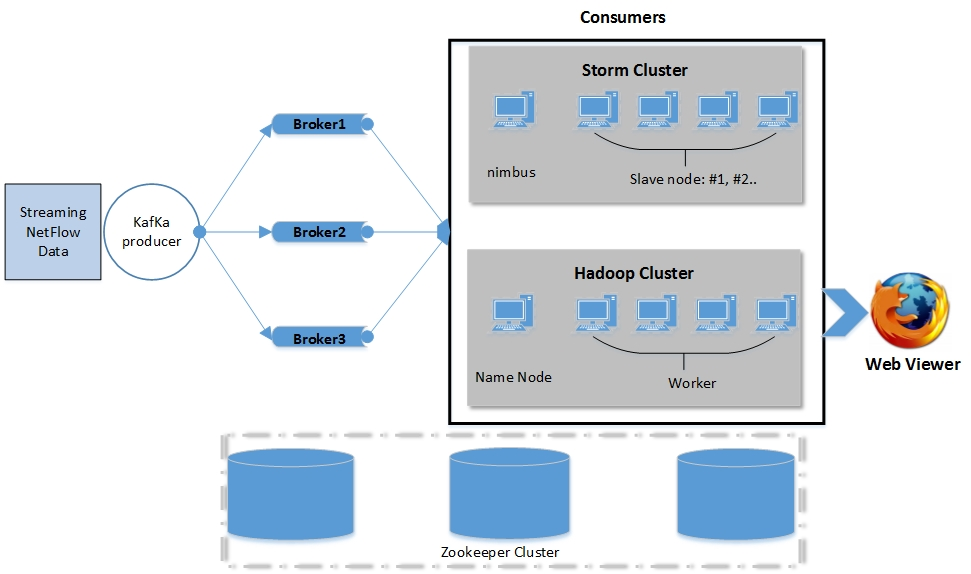
\includegraphics[scale = 0.35]{figure/arch}
%\includegraphics[width=0.3\textwidth]{figure/cibus}
\caption{Proposed Architecture}
\label{arch_drawing}
\vspace{-.1in}
\end{figure}

\section{Motivation}\label{sec:motivation}
As discussed in ~\cite{zhao2014can}, NetFlow ~\cite{netflow} data has been used as the main data source. If consider by combing different data source at different data repositories as a whole, such as campus VLAN configuration, it is very difficult to analyze network conditions when processing either history network data and real-time network data. Thus it is difficult to answer questions such as following :

\begin{enumerate}
\item What are the top high traffic applications?
	\begin{enumerate}
		\item Campus internal network traffic or external traffic
		\item What specific application, such as Youtube or Netflix
	\end {enumerate}
\item What does the current network condition look like?
	\begin{enumerate}
		\item What is the network traffic trend?
		\item If there is any abnormal activity going on.
		\end {enumerate}
\end{enumerate}



\subsection{Design}\label{sec:design}
\emph{Data model for hadoop batch processing}:

\begin{table}[h]
	\centering
	\small
	\caption{hadoop batch processing data model\{key,value\}}
	\label{table:knowledge table}
	\begin{tabular}{|l|l|}
	\hline
	Key & Value   \\\hline
	\big(sourceIP, destinationIP\big)  & Rate \big($bits/s$\big)   \\\hline
	\end{tabular}
\end{table}

\emph{Data model for real-time data processing}:

\begin{table}[h]
	\centering
	\small
	\caption{real-time processing data model \{key,value\}}
	\label{table:knowledge table}
	\begin{tabular}{|l|l|}
	\hline
	Key & Value   \\\hline
	\big(timestamp, sourceIP, destinationIP\big)  & Rate \big($bits/s$\big)   \\\hline
	\end{tabular}
\end{table}


\emph{Proposed MapReduce algothrim for history batch process using Hadoop }:

\IncMargin{1em}
\LinesNumbered
\begin{algorithm}[!ht]
    \SetKwData{U}{u}
    \SetKwData{V}{v}
    \SetKwFunction{Linkdown}{linkdown}
    \SetKwFunction{Linkup}{linkup}
    \SetKwFunction{Adj}{adj}
    \SetCommentSty{emph}
    \SetDataSty{emph}
    \SetFuncSty{emph}

    \KwIn{NetFlow Dataset $N_{f}$, Source and destination IP address \big(key, value\big) pair $IP_{src,dst}$, Bandwidth for each flow $R_{flow}$ }
    \KwOut{$\big(IP_{src,dst}$, $R_{flow}$  \big) which contains IP address and Bandwidth usage}
    \For{$f$ $\in$ $N_f$,  $ip$ $\in$ $IP_{src,dst}$}{
    		%\For{$t_c$ $\in$ $N_{t}$}{
        		\If{$ip$ in $IP_{src, dst}$}{
        			$print$ $\big(IP_{src,dst}$, $R_{flow}$  \big)
        		}
    		}
    \caption{Mapper Algorithm}
    \label{mapper_algorithm}
\end{algorithm}
\DecMargin{1em}


\IncMargin{1em}
\LinesNumbered
\begin{algorithm}[!ht]
    \SetKwData{U}{u}
    \SetKwData{V}{v}
    \SetKwFunction{Linkdown}{linkdown}
    \SetKwFunction{Linkup}{linkup}
    \SetKwFunction{Adj}{adj}
    \SetCommentSty{emph}
    \SetDataSty{emph}
    \SetFuncSty{emph}

    \KwIn{Mapper Ootput: $\big(IP_{src,dst}$, $R_{flow}$  \big) }
    \KwOut{Flows which have the most bandwidth usage,  $IP_{src,dst}$, $r_{flow}$}
	initialization  $current_{ip}=null$, $current_{rate}=0$, $previous_{rate}=0$ \;
    \For{$ip$ $\in$ $IP_{src,dst}$ , $r_{flow}$ $\in$ $R_{flow}$ }{
    		$new_{rate}$ = $r_{flow}$		\;
        		\eIf{$ip$ == $current_{ip}$ }{
        			$current_{rate}$ = $r_{flow}$ + $previous_{rate}$ 	\;
            	}{
        			$current_{ip}$ = $ip$		\;
      			$previous_{rate}$ = $current_{rate}$
            	}
            }
    	
    \caption{Reducer Algorithm}
    \label{mapper_algorithm}
\end{algorithm}
\DecMargin{1em}


\emph{Predictive recommendation model and algorithm}:


\section{Features Implemented}
\emph{network data analysis algorithms}

\emph{Prective algorithm}

\emph{WebServer User Interface}

\begin{figure}[!ht]
\centering
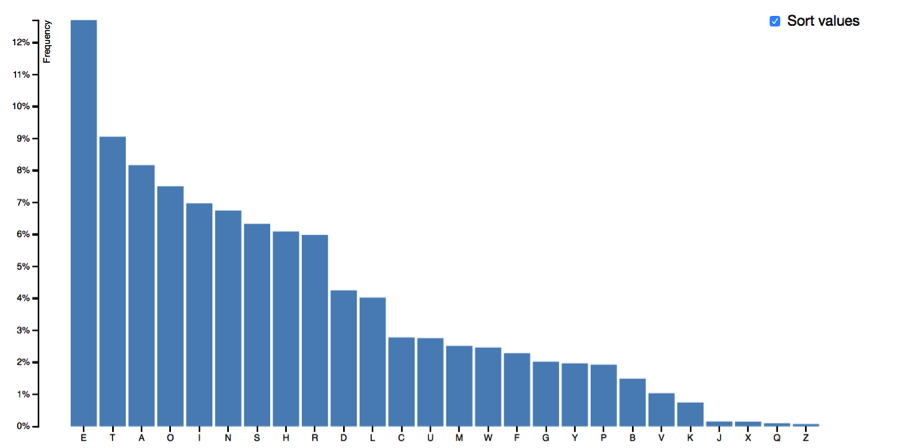
\includegraphics[scale = 0.6]{figure/sortable}
%\includegraphics[width=0.3\textwidth]{figure/cibus}
\caption{Sortable bar chart}
\label{arch_drawing}
\vspace{-.1in}
\end{figure}

\emph{Mobile User Interface}


\section{Result} label{sec:result}

\emph{History data hadoop Mapreduce}


\emph{Kafka and storm real-time}

\emph{Urls}

\begin{enumerate}
	\item Github Url: \emph{https://github.com/CS590RA/Challenge1}
	\item Hadoop Cluster Manager: \emph{http://n1.example.com:7180}
	\item Django Webserver: \emph{http://n1.exmaple.com}
	
\end{enumerate}

\section{Conclusion}\label{sec:conc}

\section{Future Work and Limitations}



\bibliographystyle{plain}
\bibliography{papers}

\end{document}


